\section{Time Trials}
Upon implementing the algorithms, we test the time-elapsed for each algorithm to see which would be best to use in practice. Each time we ran a test, the function was called using equidistant $x$ values between 0 and 1 of length $n$, B-spline regression polynomial degree 5, intercept included, and boundary knots of 0 and 1 as its parameters. The call to our function was made as follows:
\begin{verbatim}
bs(x, degree=5,intercept=TRUE, Boundary.knots=c(0,1),
   type="serial",ncls=2)
\end{verbatim}
It is important to note that the input values we used for our time trials are irrelevant. We could have used a variation of values or included internal knots but the flops count would still remain the same. Therefore, the trial inputs were kept simple but consistent to make this section easier.
\\ \\
In doing the time trials, for each length $n$, we call the respective function for either R, OpenMP, CUDA, or SNOW three times and then we took the average of the total time-elapsed. The time is measured in seconds, rounded to the thousandth decimal place.
\\ \\
The following table demonstrates the time trials with varying lengths $n$:
\begin{center}\begin{tabular}{|c||c|c|c|c|c|} \hline
n = &100& 1000& 10000& 100000& 1000000 \\ \hline \hline
R &0.015& 0.063& 0.542& 6.179& 74.425\\ \hline
OpenMP &0.004& 0.037 &0.447& 4.682& 40.562\\ \hline
CUDA &0.048 &0.084 &0.528 &4.647 &41.931\\ \hline
SNOW &0.085 &0.186 &0.358 &2.690& 21.881 \\ \hline
\end{tabular}\end{center}
In order to make it easier to view and understand the time trial results, the table can best be summarized by the following plot:


\begin{center} 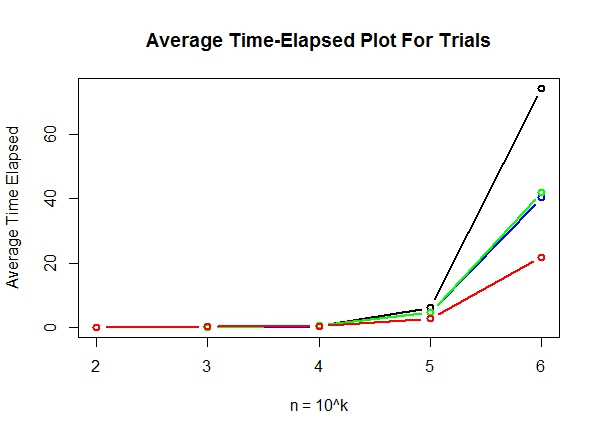
\includegraphics[scale=.5]{times.jpeg} \end{center}


A few interesting observations can be made about the time trials. In the case of OpenMP compared to serial R, when the data set approaches 10000, the difference in time decreases compared to the smaller and the larger $n$. Surprisingly, starting off much slower than both the serial R function and the OpenMP, the CUDA algorithm is significantly faster than the serial R function and on par with OpenMP as length $n$ increases. Because CUDA is essentially serial, it is possible CUDA's nvcc compiler is much more efficient than the typical GNU g++ compiler used in building OpenMP. As $n$ grows much larger, SNOW takes about half the computational time as OpenMP and CUDA, and a little more that a third of the time the serial R took.
